% AAAI 2027 author-kit format. For the anonymous review upload, change the
% package line to \usepackage[submission]{aaai2027} (authors auto-hidden).
\documentclass[letterpaper]{article}
\usepackage{aaai2027}          % official AAAI 2027 style (do not modify)
\usepackage{amsmath}
\usepackage{graphicx}
\usepackage{booktabs}
\usepackage{natbib}            % aaai2027.sty sets the aaai2027 bst itself
\frenchspacing

% AAAI defaults to unnumbered sections (secnumdepth 0); numbering is
% permitted and this paper cross-references sections, so re-enable it.
\setcounter{secnumdepth}{2}

% Figures are copied into paper/figures/ (from results/figures/) so this
% folder is self-contained for Overleaf; re-copy after regenerating results.
\graphicspath{{figures/}}

\pdfinfo{
/TemplateVersion (2027.1)
}

\title{Verify Before You Execute: A Hybrid Symbolic--Learned\\
Pre-Execution Verifier for LLM-Generated Plans}
\author{Ari Bajaj}
\affiliations{Illinois Mathematics and Science Academy\\
abajaj1@imsa.edu}

\begin{document}
\maketitle

\begin{abstract}
LLM agents increasingly emit multi-step plans---action sequences, tool-call
chains---that downstream systems execute directly. Executing a flawed plan is
costly, yet the dominant safeguards are either an LLM judging its own kind or
no check at all. We present a pre-execution verifier that translates a
free-text plan into a typed action schema, \emph{soundly} checks consistency,
goal completeness, and resource feasibility by forward simulation, and fuses
the symbolic verdict with a small calibrated \emph{trust model} that estimates
whether the NL$\to$schema translation itself was faithful. Hard symbolic
failures always reject; the trust score ranks residual translation risk. On
three domains (Blocksworld, Logistics, and a tool-use environment that reused
the pipeline with zero code changes), against oracle labels validated by two
independent simulators agreeing on 360/360 records, the hybrid attains
F1$=$0.949 at perfect recall and---most importantly---raises downstream
execute-or-reject task success from 61.1\% (no verifier) to 93.1\%, beating an
LLM-judge gate (87.5\%) because its symbolic explanations make replanning
feedback actionable. At the plan lengths typical of prior LLM-planning
benchmarks (3--8 steps), properly-budgeted LLM judges are in fact
\emph{perfect} detectors, matching the hybrid. We therefore run a
second experiment scaling plan length to 10/20/40/80 steps and find the
picture reverses: the hybrid holds F1$=$1.000 at every horizon while judge
recall degrades monotonically (0.94$\to$0.84 zero-shot, 0.92$\to$0.88
chain-of-thought), and in a live downstream execute-or-reject test at
10--20 steps the judge-gated arm lets 4--5\% of flawed plans execute while
the hybrid remains at exactly 0\% at every horizon tested---the one
guarantee sound simulation gives that judging cannot. We also report two
further negative-space findings: a constrained output format makes the
NL$\to$schema translation lossless, eliminating the trust model's target
class in that regime; and a naive token budget silently turned a fail-open
judge baseline into ``no verifier'' on 100\% of records, a deployment
failure mode worth naming on its own. Code, data generators, and all
results are reproducible from a single make target on a laptop.
\end{abstract}

\section{Introduction}

A growing class of systems lets a large language model (LLM) propose a
multi-step plan---a sequence of robot actions, API calls, or tool
invocations---and then executes that plan with little or no intermediate
checking. When the plan is flawed, the cost is paid at execution time:
side-effecting API calls fire, budgets are spent, and physical or
irreversible actions occur before the flaw surfaces. Benchmarks consistently
find that LLM plans are unreliable in exactly the ways that matter:
preconditions are violated, goal conjuncts are silently dropped, and resource
limits are exceeded \citep{valmeekam2023planbench,kambhampati2024llmmodulo}.

The natural safeguards occupy two unsatisfying extremes. Purely symbolic
validation in the style of \textsc{VAL} \citep{howey2004val} is sound but
assumes the plan already exists in a formal language---while LLM plans arrive
as free text, and the lossy translation from text to formalism becomes an
unmodeled failure source. Purely learned safeguards---asking an LLM judge
``is this plan valid?'' \citep{zheng2023judging}---inherit the fallibility
they are meant to check, and recent evidence suggests LLMs are poor
self-verifiers \citep{huang2024cannot,stechly2024selfverification}.

We study the middle: a \textbf{hybrid pre-execution verifier} for LLM plans.
An LLM extractor translates each free-text step into a typed action schema; a
sound symbolic checker forward-simulates the extracted plan and verdicts
three independent dimensions (action consistency, goal completeness, resource
feasibility); and a small calibrated \emph{trust model}---trained on
extraction confidence, $k$-resample self-consistency agreement, and
plan-shape features---estimates the probability that the symbolic verdict is
\emph{faithful} to the plan as written, i.e.\ that the translation did not
silently change what is being checked. The fusion rule is asymmetric by
design: a hard symbolic failure always rejects, regardless of trust; among
symbolic passes, low trust flags residual risk.

\paragraph{Contributions.}
(1)~A pipeline architecture and open implementation for sound pre-execution
verification of free-text LLM plans, with a learned estimate of translation
faithfulness as a first-class signal. (2)~A synthetic-data methodology with
an \emph{independent} oracle: two separately implemented simulators (labeler
and verifier) whose agreement on every record (360/360; 1{,}440/1{,}440
per-dimension comparisons) anchors all reported numbers. (3)~A generality
test: a tool-use domain (auth scopes, prerequisite calls, quotas, spend
budgets) was expressed in the same DSL and ran through the entire pipeline
with \emph{zero} code changes. (4)~A downstream execute-or-reject experiment
showing the hybrid's real edge at short horizons is not detection accuracy
but \emph{replan feedback quality}: symbolic explanations convert
rejections into successful second attempts more often than judge critiques
(5 vs.\ 9 dead-ends). (5)~A plan-length scaling experiment (10/20/40/80
steps) showing that detection accuracy parity is a short-horizon artifact:
judge recall degrades monotonically with length while sound simulation does
not, and by 10--20 steps the judge-gated downstream arm already lets
flawed plans execute at a nonzero rate that the hybrid never does.
(6)~Several honestly-reported negative and boundary results that reframe
the design space for verifier research, including a deployment failure
mode in which a fail-open LLM judge silently degrades to no verification at
all.

\section{Related Work}

\paragraph{LLM planning and its critics.}
PlanBench and successors document systematic planning failures in LLMs
\citep{valmeekam2023planbench}. The LLM-Modulo position argues LLMs should
generate while external sound modules verify \citep{kambhampati2024llmmodulo};
LLM$+$P \citep{liu2023llmp} translates problems into PDDL and delegates to a
classical planner. We keep the LLM as planner and verify its output,
targeting settings (e.g.\ tool use) where a complete classical model exists
only implicitly.

\paragraph{Plan validation.}
\textsc{VAL} \citep{howey2004val} validates PDDL2.1 \citep{fox2003pddl21}
plans against a formal domain. Our symbolic core is a deliberately small
reimplementation of this idea over a typed DSL with per-step resource
accounting; the novelty is not the checker but its coupling to a learned
model of \emph{whether the checker saw the right plan}.

\paragraph{LLM self-checking and repair.}
LLM-as-judge \citep{zheng2023judging}, Self-Refine \citep{madaan2023selfrefine},
and Reflexion \citep{shinn2023reflexion} use LLMs to critique or repair their
own outputs; \citet{huang2024cannot} and \citet{stechly2024selfverification}
find intrinsic self-correction weak on reasoning and planning. Our baselines
instantiate both judge variants and a Reflexion-style repairer on identical
inputs, and our downstream experiment measures what each safeguard is worth
at execution time.

\paragraph{Calibration and self-consistency.}
We use $k$-resample agreement in the spirit of self-consistency
\citep{wang2023selfconsistency} as a \emph{feature} rather than a decoding
rule, Platt scaling \citep{platt1999} for calibration, and expected
calibration error \citep{naeini2015ece,guo2017calibration} for evaluation.

\section{Method}

\subsection{Plan and Domain Representation}

A domain is a set of typed predicate definitions, action schemas
(preconditions, add/delete effects), and \emph{resource dimensions}---named
scalars with an initial value, a floor, and a cap, adjusted by per-action
deltas. A problem grounds a domain with typed objects, an initial state, and
a conjunctive goal. Validation is structural: an action schema may only
reference declared predicates and resources with matching arity and types.
This DSL is intentionally small---no disjunctive preconditions, conditional
effects, or typed return values---but Section~\ref{sec:tools} shows it
stretches to tool-use constraints without modification.

\subsection{Symbolic Verifier}

Given a sequence of ground actions, the verifier forward-simulates from the
initial state and emits a three-part verdict with a machine-readable
explanation:
\textbf{consistency} (every step's action exists, is well-typed, and its
preconditions hold when executed in order), \textbf{goal completeness}
(every goal conjunct holds in the final state), and \textbf{resource
feasibility} (every prefix of the running sum respects every dimension's
floor and cap). Progression is \emph{lenient}: a violated precondition is
recorded but effects still apply, so one early slip cannot mask an
independent later flaw---each dimension verdicts independently. Upstream
parse or extraction failures are injected as consistency violations, since an
executor could not run those steps. \texttt{overall\_valid} is the
conjunction of the three checks.

\subsection{NL$\to$Schema Extraction with Self-Consistency}

Free-text steps are mapped to ground actions by an LLM extractor using the
API's structured-output mode, validated against the domain (action name,
arity, object types). On validation failure the extractor retries once with
the error as feedback, then falls back to a null extraction with confidence
$0$---it never crashes, it degrades. Each step is resampled $k{=}3$ times at
temperature 0.7; the modal extraction is used, and two agreement statistics
(exact-match fraction and action-type-match fraction) are retained. These,
with the extractor's self-reported confidence, become features rather than
being discarded.

\subsection{Trust Model and Fusion}
\label{sec:trust}

The trust model answers: \emph{given how the extraction went, how likely is
the symbolic verdict faithful to the plan as written?} Its label is
agreement between the production verdict (LLM extraction path) and a
reference verdict computed by a deterministic rule-based parse of the
original plan text. Features (17) span extraction confidence (mean/min),
$k$-resample agreement, plan-shape statistics, the fraction of
failed-extraction steps, a TF-IDF character-$n$-gram similarity between the
preconditions the extractor \emph{mentioned} and those the schema
\emph{requires}, the symbolic verdict bits and violation counts, and a
domain indicator. The classifier is a class-balanced logistic regression,
Platt-scaled on a held-out validation split; all splits are by
\emph{problem}, so no problem's records straddle train/test.

Fusion is a two-clause rule with a tested invariant:
\[
\textbf{reject} \iff \neg\text{symbolic\_valid} \;\lor\; \text{trust} < \tau,
\]
where the first clause is unconditional---no trust score can rescue a hard
symbolic failure---and $\tau$ is picked on validation. $\tau{=}0$ recovers
symbolic-only exactly.

\section{Experimental Setup}

\subsection{Domains, Problems, and Gold Plans}

\textbf{Blocksworld} (4 operators $+$ a crane-energy resource),
\textbf{Logistics} (trucks/planes over two cities, fuel $+$ budget), and
\textbf{Tools} (Section~\ref{sec:tools}). A seeded generator produces
problems whose BFS-optimal gold plans span 3--8 steps; determinism is
enforced cross-process (a \texttt{PYTHONHASHSEED} ordering bug found by a
subprocess test motivated sorting all set-derived output). Resource caps are
tightened to $\lceil 1.25\times\rceil$ the gold plan's consumption so that
wasteful plans can actually overrun.

\subsection{Long-Horizon Problems}
\label{sec:horizonsetup}

Prior LLM-planning benchmarks concentrate on short plans, and our own
main dataset (3--8 steps) is no exception---raising the question of
whether any detector comparison run at that length generalizes. To test
this directly we build a second, constructive generator per domain
(BFS gold-planning is infeasible past $\sim$10 steps) that scales problem
size (blocks, packages, trips) to hit nominal horizons of 10, 20, 40, and
80 reference-plan steps: Blocksworld tears every tower down to the table
and rebuilds the goal arrangement bottom-up; Logistics routes each package
sequentially through its truck/airport/plane legs; Tools authenticates each
needed scope once and executes every trip's milestone prerequisite chain in
order. Every constructive plan is independently strict-simulated at
generation time and re-checked by the oracle labeler, so a bug in a
constructive planner cannot silently ship an invalid reference plan; the
one honest caveat is that these plans are valid but \emph{not optimal}
(Blocksworld especially), so ``horizon $H$'' denotes a band on the
reference length, not an optimality claim. To bound API cost, the
$k$-resampled extraction path runs on all 40 records per horizon at
$H{\in}\{10,20\}$ but on a stratified 12-record subset at
$H{\in}\{40,80\}$; judges and self-repair run on all records at every
horizon. Token budgets were raised throughout (generation/paraphrase to
4{,}096, judges/self-repair to 8{,}192 tokens) so long plans are not
silently truncated the way Section~\ref{sec:budget} describes.

\subsection{Plan Generation with Failure Injection}

For each problem, \texttt{claude-haiku-4-5} (temperature 1.0) writes a plan
under four prompt conditions: \emph{baseline} (honest prompt),
\emph{goal-omission} (one goal conjunct silently dropped from the prompt;
labels use the full goal), \emph{resource-blind} (limits stripped), and
\emph{distractor} (plausible invalid actions offered). A pilot calibration
confirmed the conditions amplify naturally occurring failure modes rather
than inject alien ones: 43--47\% of \emph{baseline} plans are already
flawed, and goal-omission roughly quadruples goal-incompleteness. Dataset:
3 domains $\times$ 30 problems $\times$ 4 conditions $=$ 360 records.

\subsection{Independent Oracle and Soundness Evidence}

Ground-truth labels come from an oracle labeler that is a \emph{separate
implementation} of plan simulation from the verifier (shared design
semantics, disjoint code). Agreement between the two on rule-parsed plans is
therefore evidence, not tautology: across all 360 records they agree on
overall validity 360/360 and on all 1{,}440 per-dimension comparisons, with
every flaw type additionally covered by hand-verified adversarial fixtures.
The evaluation CLI recomputes this cross-check on every run and fails loudly
on any disagreement.

\subsection{The Prose Regime}
\label{sec:prose}

Our first finding is methodological: with a constrained output format
(\texttt{Step $N$: action(args)}), the LLM extraction path's verdict agreed
with the rule-based reference on \textbf{240/240} records---the
NL$\to$schema translation was lossless, the trust label had one class, and
the learned layer had nothing to model. This is a genuine scoping result:
\emph{where plans can be forced into a rigid format, a rule parser plus a
sound checker suffices}. To study the setting the trust model exists for,
the production pipeline verifies an LLM-generated \emph{prose paraphrase} of
each plan (one sentence per step, no rigid syntax), while labels stay
anchored to the original constrained text. In the prose regime 13/360
records (3.6\%) get unfaithful verdicts---sparse, but a real target class.

\subsection{Baselines}

On identical prose inputs: \textbf{LLM judge} (zero-shot and
chain-of-thought, verdict parsed from a required \texttt{VERDICT:} line,
fail-open on unparseable output, mirroring naive deployment);
\textbf{symbolic-only} ($\tau{=}0$); \textbf{learned-only} (the trust
feature vector with all five symbolic-verdict features removed, trained to
predict validity directly---the no-grounding ablation); and
\textbf{self-repair} (Reflexion-style single-pass critique$+$rewrite
\citep{shinn2023reflexion}, with change-detection standing in for a verdict).

\subsection{Metrics}

Positive class $=$ \emph{flawed plan}; rejecting is a positive prediction.
We report P/R/F1 overall, per domain, and per flaw type; ECE with
reliability diagrams for the trust model; API-call and local-latency cost
proxies; and the downstream experiment of
Section~\ref{sec:downstream}. Test split: 72 records (problem-level,
216/72/72).

\section{Results}

\subsection{Detection}

\begin{table}[t]
\centering
\small
\begin{tabular}{lccc}
\toprule
System & P & R & F1 \\
\midrule
Hybrid (ours, $\tau$ picked on val) & 0.903 & \textbf{1.000} & 0.949 \\
Symbolic-only & 0.903 & \textbf{1.000} & 0.949 \\
Learned-only (no symbolic feats) & 0.618 & 0.750 & 0.677 \\
LLM judge, zero-shot & \textbf{1.000} & \textbf{1.000} & \textbf{1.000} \\
LLM judge, CoT & \textbf{1.000} & \textbf{1.000} & \textbf{1.000} \\
Self-repair (change detection) & 0.966 & \textbf{1.000} & 0.982 \\
\bottomrule
\end{tabular}
\caption{Detection on the 72-record pooled test split (positive class $=$
flawed). Per-flaw recall for the hybrid: 20/20 inconsistency, 10/10
goal-incompleteness, 5/5 resource-infeasibility.}
\label{tab:main}
\end{table}

Table~\ref{tab:main} contains a result we report at full prominence:
\textbf{both LLM judges are perfect on this test split}. Plans of 3--8
steps are short enough for the judge model to simulate flawlessly when
given an adequate token budget (see Section~\ref{sec:budget}). At this
horizon, ``hybrid beats LLM-judge on detection'' is \emph{not supported}
by Table~\ref{tab:main} alone---but Section~\ref{sec:horizon} shows this
parity is a short-horizon artifact that does not survive longer plans. The
learned-only ablation (F1 0.677) confirms the symbolic grounding carries
the detection signal.

The hybrid's only errors are 3 false rejects, all on the Tools domain
(precision there 0.833, perfect elsewhere), all with one signature: the
extractor mangles hyphenated arguments (\texttt{flights-scope} $\to$
\texttt{flights}), producing unknown-object violations on genuinely valid
plans.

\subsection{Detection Parity Is a Short-Horizon Artifact}
\label{sec:horizon}

\begin{table}[t]
\centering
\small
\setlength{\tabcolsep}{4pt}
\begin{tabular}{lccc}
\toprule
Horizon & Hybrid F1 & Judge-zs F1 (R) & Judge-CoT F1 (R) \\
\midrule
5 (ref.) & 0.949 & 1.000 (1.00) & 1.000 (1.00) \\
10 & \textbf{1.000} & 0.967 (0.94) & 0.960 (0.92) \\
20 & \textbf{1.000} & 0.950 (0.91) & 0.976 (0.95) \\
40 & \textbf{1.000} & 0.937 (0.88) & 0.962 (0.93) \\
80 & \textbf{1.000} & 0.914 (0.84) & 0.938 (0.88) \\
\bottomrule
\end{tabular}
\caption{F1 (and recall in parentheses for the judges) vs.\ nominal plan
horizon, pooled over domains. The hybrid is perfect at every horizon
$\geq{}$10; judge recall degrades monotonically as plans lengthen.}
\label{tab:horizon}
\end{table}

We repeat detection at nominal horizons of 10, 20, 40, and 80 steps
(Section~\ref{sec:horizonsetup}). Table~\ref{tab:horizon} settles the
question Section~\ref{sec:trustresult}'s parity result left open: the
hybrid (identical to symbolic-only at every horizon tested, since
$\tau{=}0$ throughout) holds F1$=$1.000 and recall$=$1.000 at every horizon
from 10 to 80 steps---expected, since forward simulation's cost is linear
in plan length and its correctness does not degrade with length. Both
judges degrade monotonically in \emph{recall} as horizon grows (zero-shot
1.00$\to$0.94$\to$0.91$\to$0.88$\to$0.84; CoT 1.00$\to$0.92$\to$0.95$\to$
0.93$\to$0.88, noisier but the same downward drift,
Figure~\ref{fig:recall_horizon})---they increasingly fail to \emph{catch}
flawed plans, not fail to parse: judge mean output tokens rise with horizon
(zero-shot 634$\to$854, CoT 765$\to$1{,}192 tokens,
Figure~\ref{fig:judge_tokens}) and 0/480 judge calls were unparseable at
any horizon, so this is a genuine simulation-accuracy failure, not a
formatting artifact. The flaw rate among LLM-generated plans also rises
sharply with horizon (38.9\% at $H{=}5$ $\to$ 65\% at $H{=}10$ $\to$ 87.5\%
at $H{=}20$ $\to$ 100\% at $H{=}80$)---longer LLM-generated plans are both
harder to verify \emph{and} more likely to be flawed, compounding the value
of a sound checker exactly where judges get worse.

\begin{figure}[t]
\centering
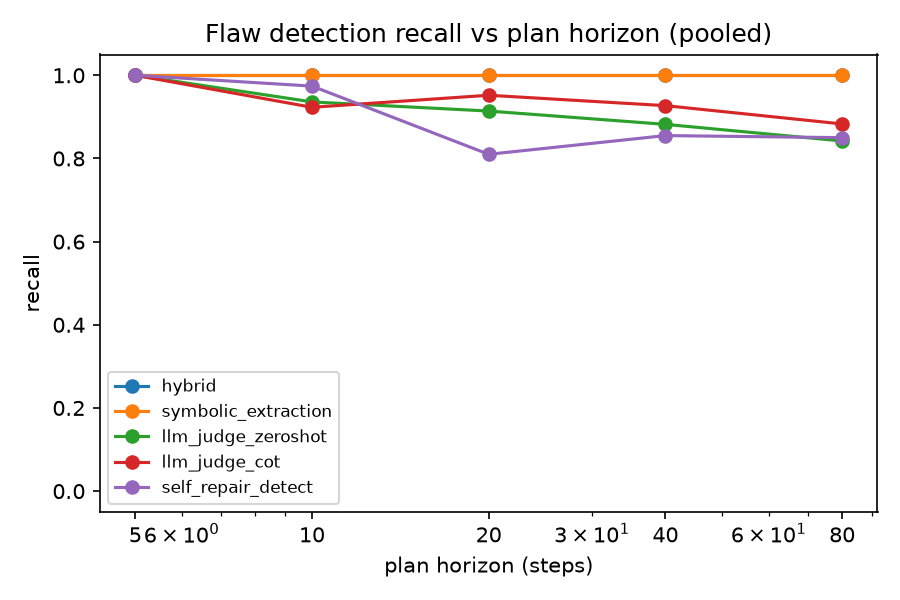
\includegraphics[width=0.95\columnwidth]{recall_vs_horizon.png}
\caption{Flaw-detection recall vs.\ plan horizon, pooled. The hybrid stays
at 1.0; both judges drift downward as plans lengthen.}
\label{fig:recall_horizon}
\end{figure}

The soundness gap this implies is not merely theoretical: we re-ran the
downstream execute-or-reject experiment (Section~\ref{sec:downstream}) at
$H{\in}\{10,20\}$ (120 records each; $H{=}40,80$ were not affordable to run
downstream given the recall trend already visible at $H{\leq}20$). At
$H{=}5$ both gates achieved 0\% executed-flawed. At $H{=}10$ the
judge-gated arm lets \textbf{5\%} of records execute a flawed plan despite
the gate; at $H{=}20$, \textbf{4.2\%}. The hybrid-gated arm remains at
\textbf{exactly 0\%} executed-flawed at both horizons---the one guarantee
sound simulation gives that judging cannot, and the guarantee actually
degrades under exactly the conditions (longer, more complex, more
failure-prone plans) where a verifier is needed most. Task success falls
for every arm as horizon grows (the underlying planner LLM struggles at
10--20 steps, independent of verification), but the hybrid still leads at
both horizons (0.667 vs.\ 0.525 at $H{=}10$; 0.383 vs.\ 0.283 at $H{=}20$).
We flag two limits on this result honestly: the long-horizon extraction
cells are 12-record stratified subsets with correspondingly wide error
bars, and the constructive gold plans are valid but not optimal
(Section~\ref{sec:horizonsetup}).

\begin{figure}[t]
\centering
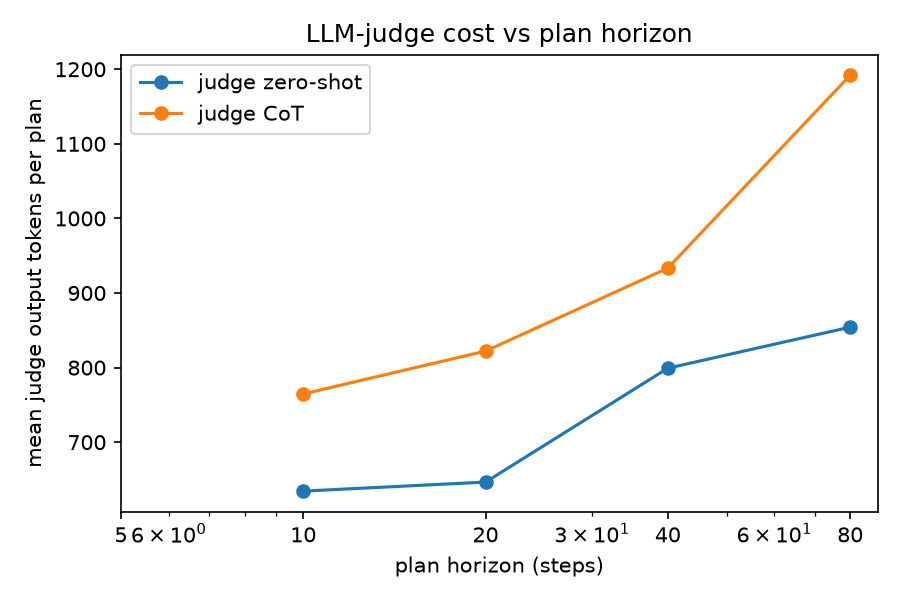
\includegraphics[width=0.95\columnwidth]{judge_tokens_vs_horizon.png}
\caption{Mean judge output tokens vs.\ plan horizon. Judges spend more
compute on longer plans yet still miss more flaws (Table~\ref{tab:horizon}).}
\label{fig:judge_tokens}
\end{figure}

\subsection{The Trust Signal Points the Right Way---but the Fusion Rule
Cannot Use It}
\label{sec:trustresult}

The validation-picked threshold is $\tau{=}0$: the trust layer never
changes a decision at dev scale, and the test split contains zero
symbolically-clean-but-flawed records for it to catch (41 symbolic passes,
all genuinely valid). Yet the signal itself is demonstrably real: the three
false-rejected mistranslations receive the trust model's \emph{lowest}
scores in the entire test split (0.74--0.82, vs.\ $>$0.9 elsewhere;
classifier accuracy 0.958, ECE 0.067, Figure~\ref{fig:reliability}). The
model detects unfaithful translation exactly as designed---but our fusion
rule, like prior gate-then-execute designs, only lets trust \emph{add}
rejections. A bidirectional rule (low-trust symbolic reject $\to$
re-extract, or fall back to the rule parser) would have repaired all three
errors and is the concrete architectural lesson of this study.

\begin{figure}[t]
\centering
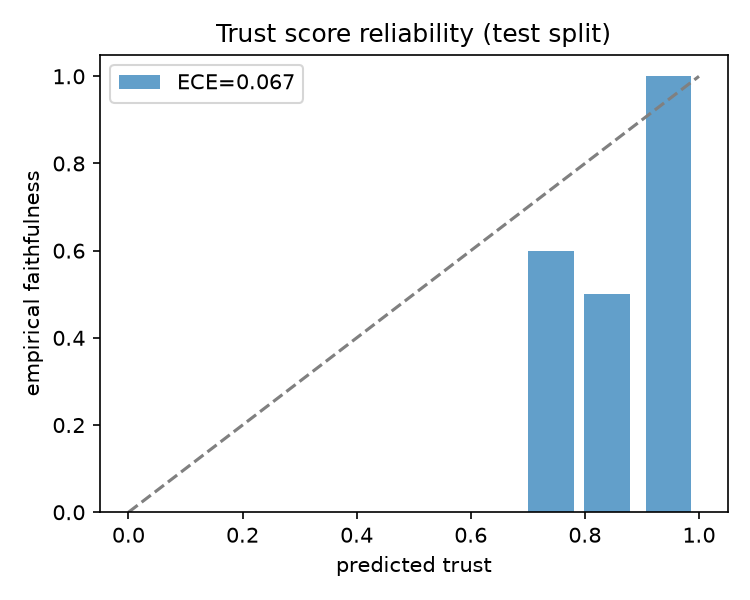
\includegraphics[width=0.95\columnwidth]{reliability.png}
\caption{Trust-model reliability diagram (test split). Mass concentrates in
the top bin at accuracy 1.0; the sparse low-confidence bins are exactly the
mistranslated records of Section~\ref{sec:trustresult}.}
\label{fig:reliability}
\end{figure}

\begin{figure}[t]
\centering
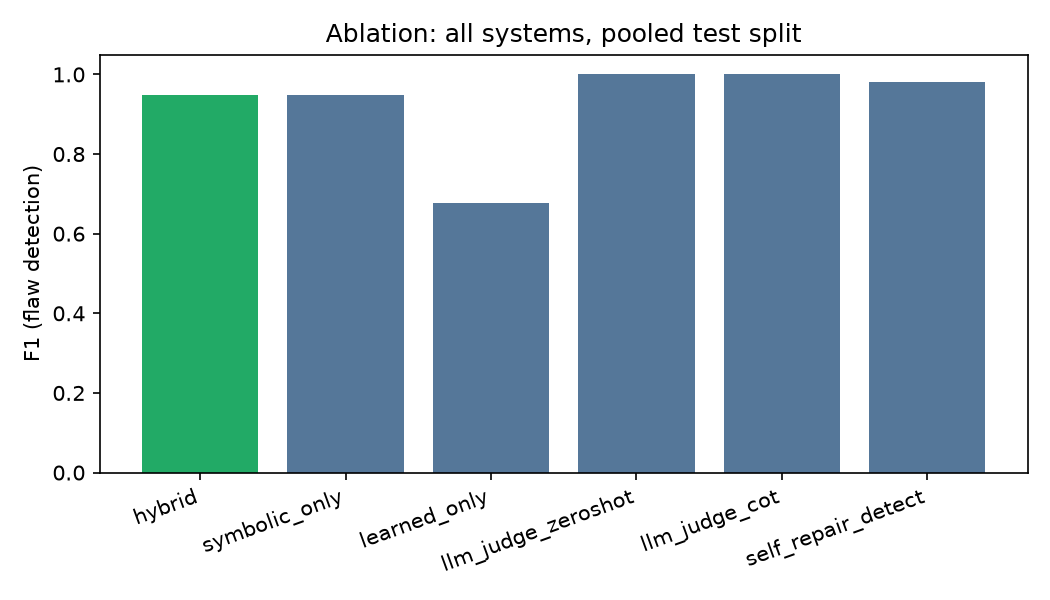
\includegraphics[width=0.95\columnwidth]{ablation.png}
\caption{F1 by system and domain. The learned-only bar shows the cost of
removing symbolic grounding; judge bars are at ceiling at this plan length.}
\label{fig:ablation}
\end{figure}

\subsection{Downstream: Execute or Reject}
\label{sec:downstream}

\begin{table}[t]
\centering
\small
\setlength{\tabcolsep}{3pt}
\begin{tabular}{lcccc}
\toprule
Arm & Success & Flawed exec. & Replans & Dead ends \\
\midrule
No verifier & 0.611 & 0.389 & 0 & 0 \\
Hybrid-gated & \textbf{0.931} & \textbf{0.000} & 31 & \textbf{5} \\
CoT-judge-gated & 0.875 & \textbf{0.000} & 28 & 9 \\
\bottomrule
\end{tabular}
\caption{Execute-or-reject with one feedback-driven replan (72 test
records). Success $=$ an executed plan that is actually valid.}
\label{tab:downstream}
\end{table}

Table~\ref{tab:downstream} is where the architecture earns its keep at this
horizon. Both gates eliminate flawed execution entirely here, but the
hybrid converts more rejections into successful second attempts: its
replan feedback is the symbolic explanation itself (``step 3: unknown
object \dots'', ``goal conjunct \texttt{on(b3,b2)} unmet''), which is more
actionable than the judge's free-text critique---5 vs.\ 9 dead-ends, 93.1\%
vs.\ 87.5\% final task success. At $H{=}5$: detection parity, feedback
superiority. Section~\ref{sec:horizon} reruns this exact experiment at
longer horizons and finds the judge's ``eliminates flawed execution
entirely'' property itself breaks down.

\subsection{A Deployment Failure Mode: the Silently Absent Judge}
\label{sec:budget}

Our first zero-shot judge used a 64-token budget, reasoning that a
one-line verdict needs no more. The judge model ignored the ``respond with
exactly one line'' instruction, simulated the plan step by step, and was
truncated before ever emitting its verdict---on \textbf{360/360 records}.
Because unparseable output fails open (as a naive deployment would), the
judge scored P$=$R$=$0.0 while appearing to run normally: the system
silently became \emph{no verifier at all}. At 512 tokens, 41\% of outputs
still truncated; only at 2{,}048 (the CoT budget) did parse failures reach
zero---whereupon the judge jumped from 0.0 to a perfect 1.0. We fixed the
baseline and report the fixed numbers, but the episode is itself a finding:
fail-open verdict parsing plus format non-compliance is a silent
total-failure mode, and the zs-vs-CoT contrast in any judge comparison is
confounded by budget unless equalized.

\subsection{Self-Repair and Cost}

The Reflexion-style repairer is a surprisingly strong \emph{fixer}---23/28
flawed plans repaired, 0/44 valid plans broken---but an unreliable
\emph{detector} (change-detection conflates cosmetic rewrites with flaw
detection). Cost: the symbolic path decides in ${\sim}0.2\,\mu$s locally
with zero API calls; the hybrid adds $k{\times}$steps extraction calls
(${\sim}$12--24, batchable); each judge call generates up to 2{,}048
tokens. A verifier that is free at decision time changes how often one can
afford to check.

\subsection{Generality: the Tool-Use Domain}
\label{sec:tools}

The Tools domain models a travel-booking agent: eight tools, auth scopes as
predicates, prerequisite calls threaded as boolean return-value facts
(\texttt{search\_flights} adds \texttt{flight-options(trip)}, which
\texttt{book\_flight} requires), an API quota ($-1$/call) and a spend
budget (flight 300, hotel 200) as resource dimensions. \textbf{No changes
to any pipeline code were required}---the same labeler, verifier,
extractor, and trust model ran as-is, and the domain's verdicts cross-check
120/120 against the oracle. The one representational wrinkle: the DSL lacks
constant action arguments, so scopes are pinned by identity predicates.
Notably, the pipeline's only false rejects arise here, from hyphenated
tool-argument extraction---evidence that tool-style vocabularies stress the
NL$\to$schema seam more than classical planning vocabularies do.

\section{Limitations}

All numbers are dev-scale: 360 short-horizon records (72-record test
split, 13 negative trust labels) plus 12 records per domain per long
horizon at $H{\in}\{40,80\}$ (wide error bars there), one model family
(\texttt{claude-haiku-4-5}) for every LLM role, single seed. The
long-horizon gold plans are valid but not optimal
(Section~\ref{sec:horizonsetup}), so ``horizon $H$'' is a nominal band, not
an optimality claim, and the downstream soundness-gap result
(Section~\ref{sec:horizon}) is demonstrated only at $H{\leq}20$, not yet at
$H{=}40,80$ where the recall trend suggests it would be larger. The trust
layer's value proposition is confined to the prose regime by construction
(Section~\ref{sec:prose}); the paraphrase step can itself add label noise
(all systems see identical text, so comparisons stay like-for-like). The
oracle and verifier share design semantics though not code, so a shared
semantic error would evade the cross-check; hand-verified fixtures and
(future) \textsc{VAL} \citep{howey2004val} validation are the defenses.
Precondition similarity is lexical; the DSL omits conditional effects and
typed return values; the downstream replan arm is gated by the sound
rule-based check, so its ``accepted implies valid'' property is by
construction and the informative quantities are replan success and
ungated flawed-execution cost. A remaining open question worth naming
plainly: the near-100\% extraction-fidelity rate at $H{\geq}10$
(Section~\ref{sec:horizon}) measures agreement between two extraction
paths on mechanically repetitive long-horizon plans, not ground-truth
extraction accuracy, and should not be read as translation becoming more
reliable with plan length.

\section{Conclusion}

We built and honestly evaluated a hybrid pre-execution verifier for
free-text LLM plans. At short horizons (3--8 steps, the range typical of
prior LLM-planning benchmarks) its detection matches a sound symbolic check
and is beaten to ceiling by a well-budgeted LLM judge---but even there it
wins where execution happens: the highest downstream task success (93.1\%)
and replan feedback that turns rejections into successes more often. That
short-horizon parity, however, does not survive scale: at 10--80 steps the
hybrid remains perfect while judge recall degrades monotonically, and by
10--20 steps the judge-gated downstream arm already lets flawed plans
execute at a nonzero rate the hybrid never does. Four findings reframe the
design space: sound verification is a length-invariant guarantee that LLM
judging is not, and the gap opens exactly where plans get harder and more
error-prone; constrained formats make translation lossless (making the
trust problem vanish where they are available); trust signals should flow
\emph{both} ways through the fusion rule, triggering re-extraction rather
than only extra rejection; and fail-open judge deployments can silently
become no verifier at all. The obvious next step is to push the downstream
soundness-gap measurement to 40--80 steps and to real (non-synthetic)
long-horizon planning tasks, where we expect the gap this laptop-scale
infrastructure surfaced to widen further.

\section*{Reproducibility}

All code, domain generators, prompts, and evaluation scripts are in the
project repository; \texttt{make reproduce} regenerates every number and
figure in this paper from fixed seeds (\texttt{make reproduce FULL=1} for
the full-scale configuration). Datasets are synthesized locally; the only
external dependency is an Anthropic API key.

\bibliography{references}

\end{document}